\section{Simulation of local NPI implementation during Victoria's second wave}

\subsection{School closures}
The effect of Victorian school closures is captured through the timeline presented in Table \ref{tab:school_timeline}.


\begin{table}[ht]
\renewcommand{\baselinestretch}{1}
	\begin{tabular}[ht]{| p{4.2cm} | p{6.2cm} | p{3.2cm} |}
	\hline
		Date of change & Policy change & Modification applied to school contacts contribution to mixing matrix, \(s(t)\) \\
		\hline
		From model start & Remote learning & 0.1 \\
		\hline
		26\textsuperscript{th} May & 400,000 school students return to school & 0.393 \\
		\hline
		9\textsuperscript{th} June & Remaining 618,000 school students return to school & 1 \\
		\hline
		9\textsuperscript{th} July & Remote learning for stage 3 restrictions & 0.1 \\
		\hline
    \end{tabular}
    \caption{Timeline used to implement Victorian school closure policies. The function is applied to both metropolitan and regional clusters.}	
    \label{tab:school_timeline}
\end{table}

\subsection{Macrodistancing in workplaces and other locations}
The functions applied here are determined by the Google mobility data according to Table \ref{tab:mobility_map}, as described above, but are applied separately for each cluster. Because Google mobility data pertains to local government areas (LGAs), whereas health service clusters may receive patients from across the state, it was necessary to map mobility data to clusters. Health service clusters' overall mobility values in each location were calculated using a weighted average of LGA mobility values according to the historical pattern of the origin of patients presenting to services within each cluster.

As a hypothetical example, if 50\% of patients historically presenting to Barwon South West health cluster services come from the City of Geelong, the mobility data for the City of Geelong will contribute 50\% of the Google mobility estimate of Barwon South West.

Historical patterns of patient presentations by health service cluster were provided by the Victorian Department of Health and Human Services (DHHS).

\subsection{Microdistancing approach}
In this application to Victoria, the microdistancing function \(m(t)\) is comprised of two components: physical distancing and face coverings. Both physical distancing and face coverings micro-distancing are applied to the three non-household locations, such that the microdistancing function for non-household locations is given by: \[m(t)=d(t)^2\times f(t)^2\]
The two interventions are assumed to be independent and so are multiplicative. As for the macrodistancing functions, the two functions of time are squared to represent their effects on both the infector and the infectee in any potentially infectious interaction.

\subsection{Physical distancing}
The physical distancing function \(d(t)\) is a transposed and translated hyerbolic tan function. The parameters of this function were estimated by using maximum a posteriori inference, with priors that penalised large shape parameters (to avoid extremely rapid transitions). The proportions of respondents answering ``always" to YouGov surveys of Victorian residents asking ``Thinking about the last 7 days, about how many people from your household have you come into physical contact with (within 2 meters / 6 feet)?" were used as input data. Resulting parameters were: shape, 0.262764; lower asymptote, 0.2803973; upper asymptote; 0.4421819; and inflection point, 15\textsuperscript{th} July. The resulting function is presented in Figure \ref{fig:physical}.

\begin{figure}[ht]
    \resizebox{1\textwidth}{!}{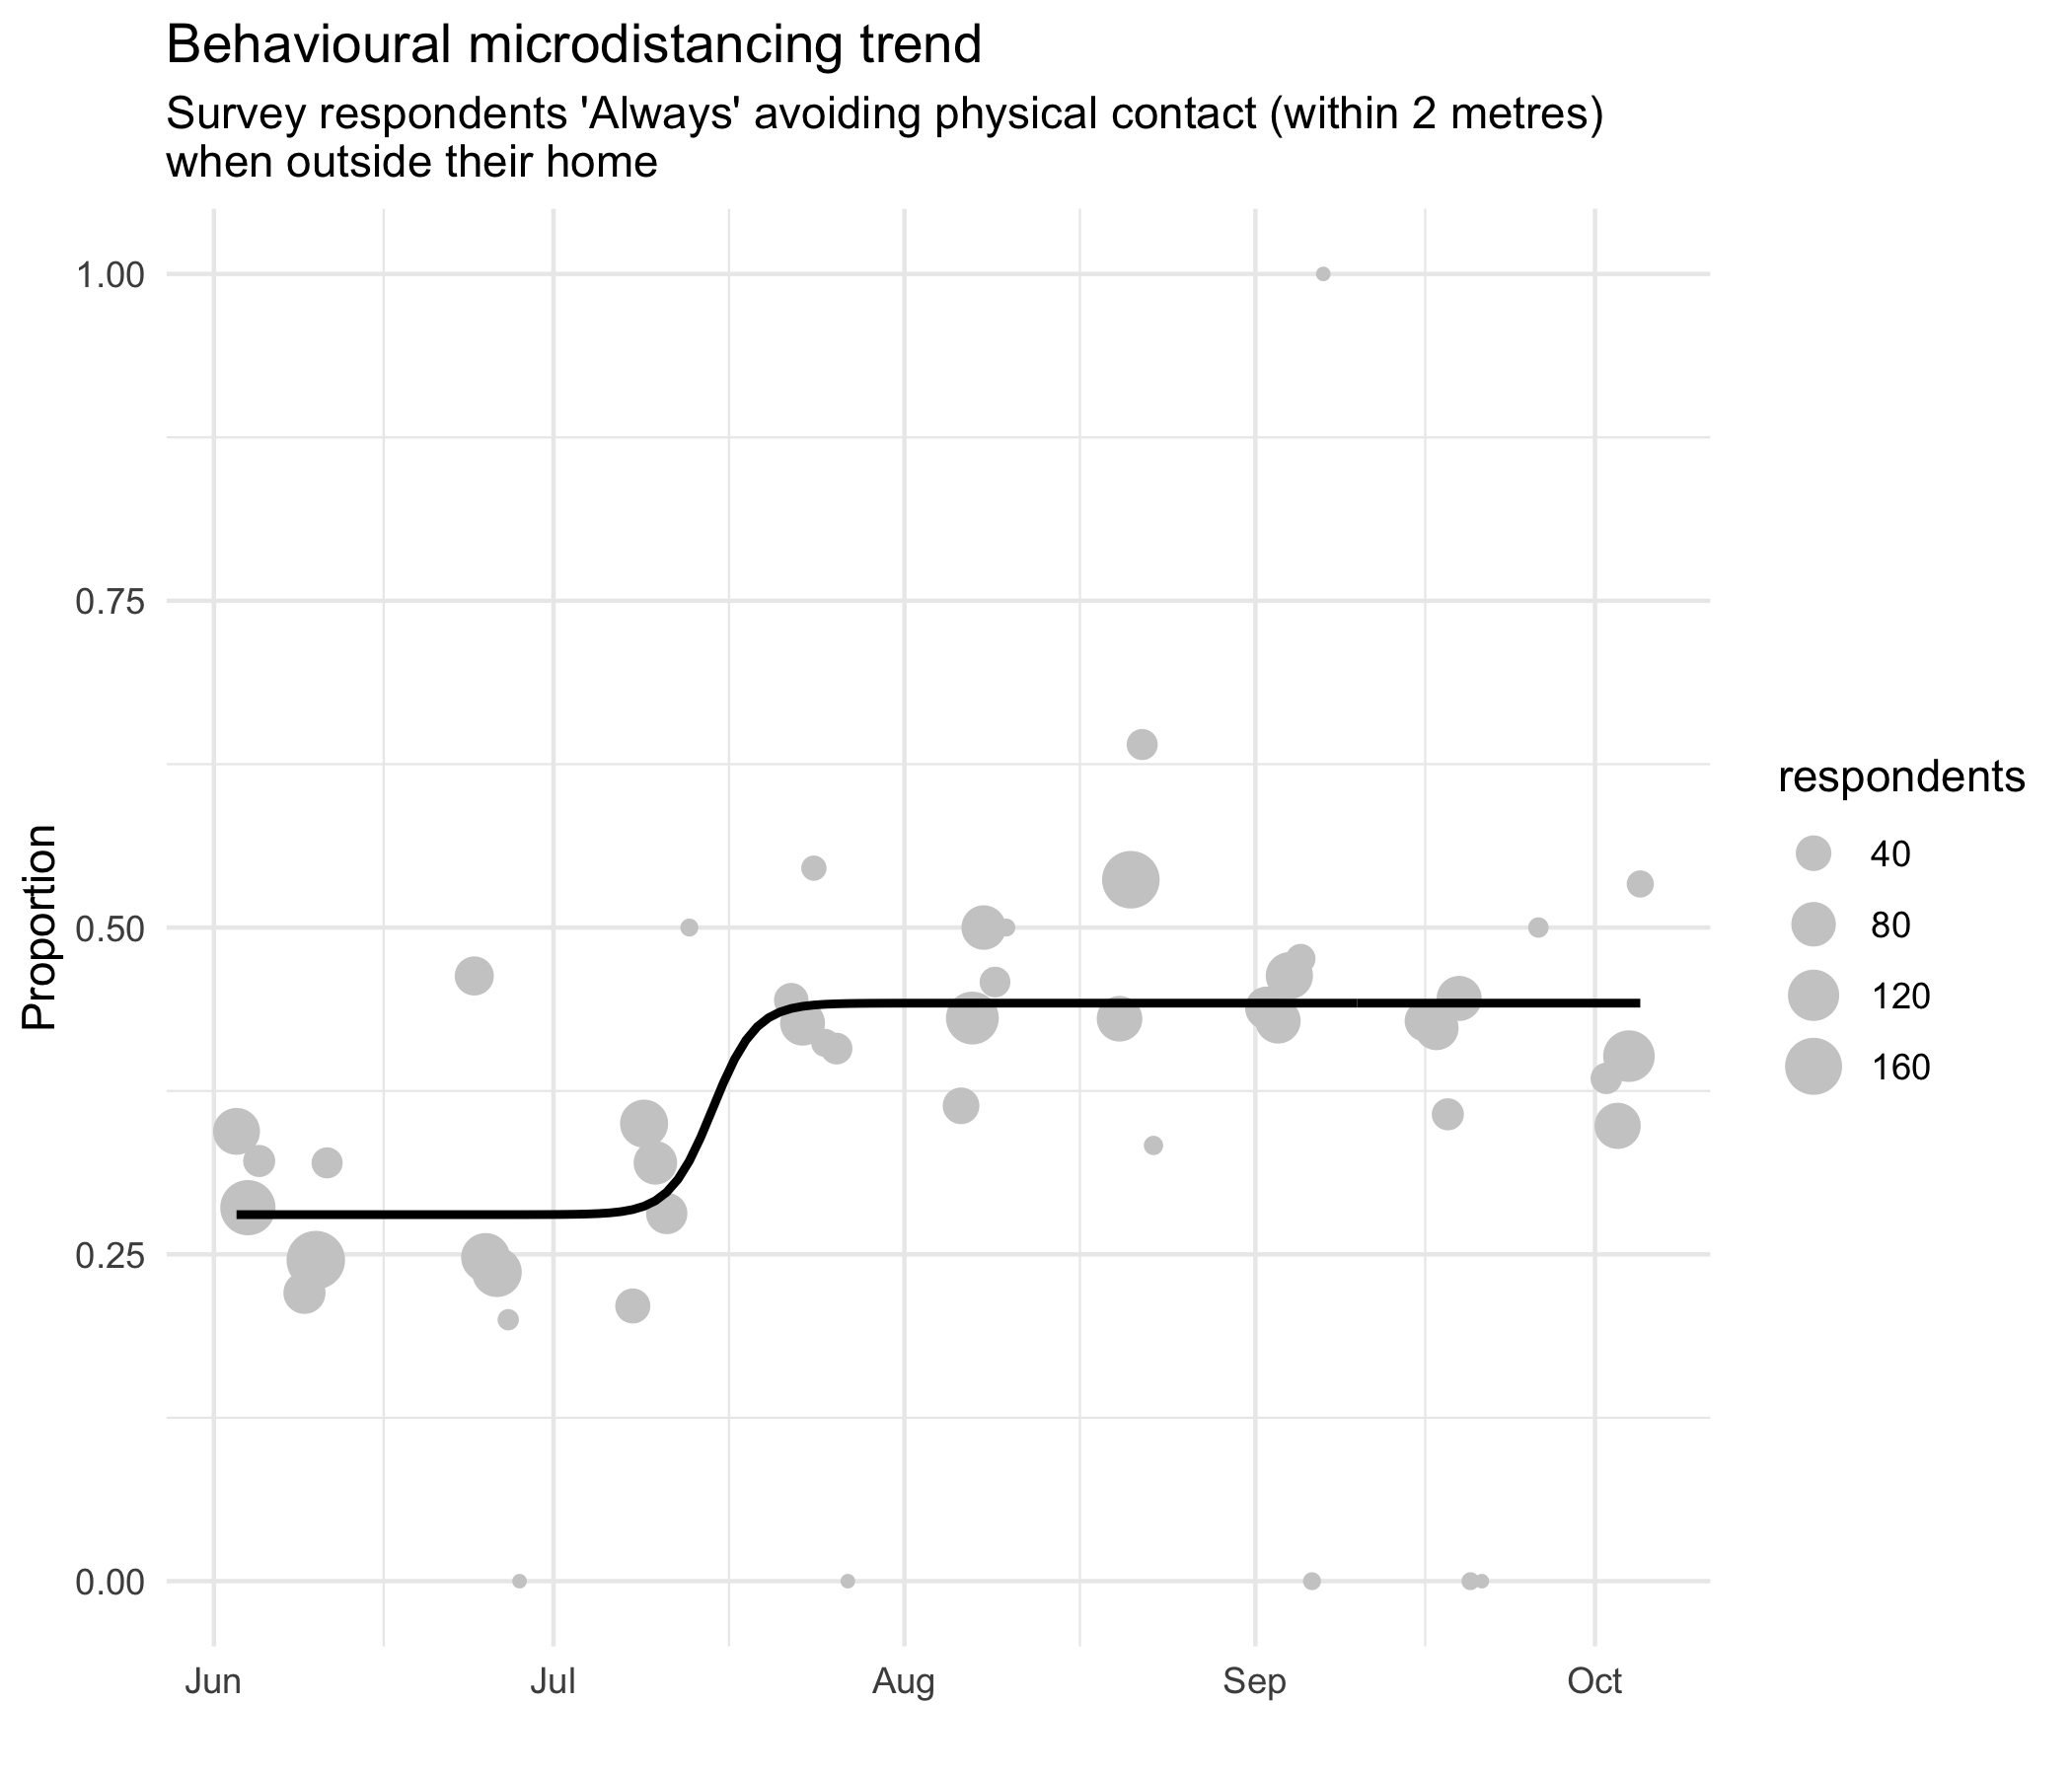
\includegraphics[scale=1]{../covid_19/projects/victoria/methods_figures/physical_distancing_fig.png}}
    \caption{Physical distancing micro-distancing function (for all clusters) with data used for fitting.}
    \label{fig:physical}
\end{figure}

\subsection{Face coverings}
Two separate face coverings microdistancing functions are employed, one for metropolitan and one for regional health service clusters. These functions were fitted using the same methods as for physical distancing, using YouGov data on Victorian residents' survey responses to the question ``Thinking about the last 7 days, have you worn a face mask outside your home (e.g. when on public transport, going to a supermarket, going to a main road)?". Estimated parameters were: shape, 0.5261693; lower asymptote, 0.130469; upper asymptote, 0.9143849; and inflection point, 23\textsuperscript{rd} July (consistent with the policy change in metropolitan Melbourne). This was applied directly to metropolitan clusters and translated ten days later for regional clusters, where face coverings were mandated from the 2\textsuperscript{nd} August. The resulting function is presented in Figure \ref{fig:face}.

\begin{figure}[ht]
 	\resizebox{1\textwidth}{!}{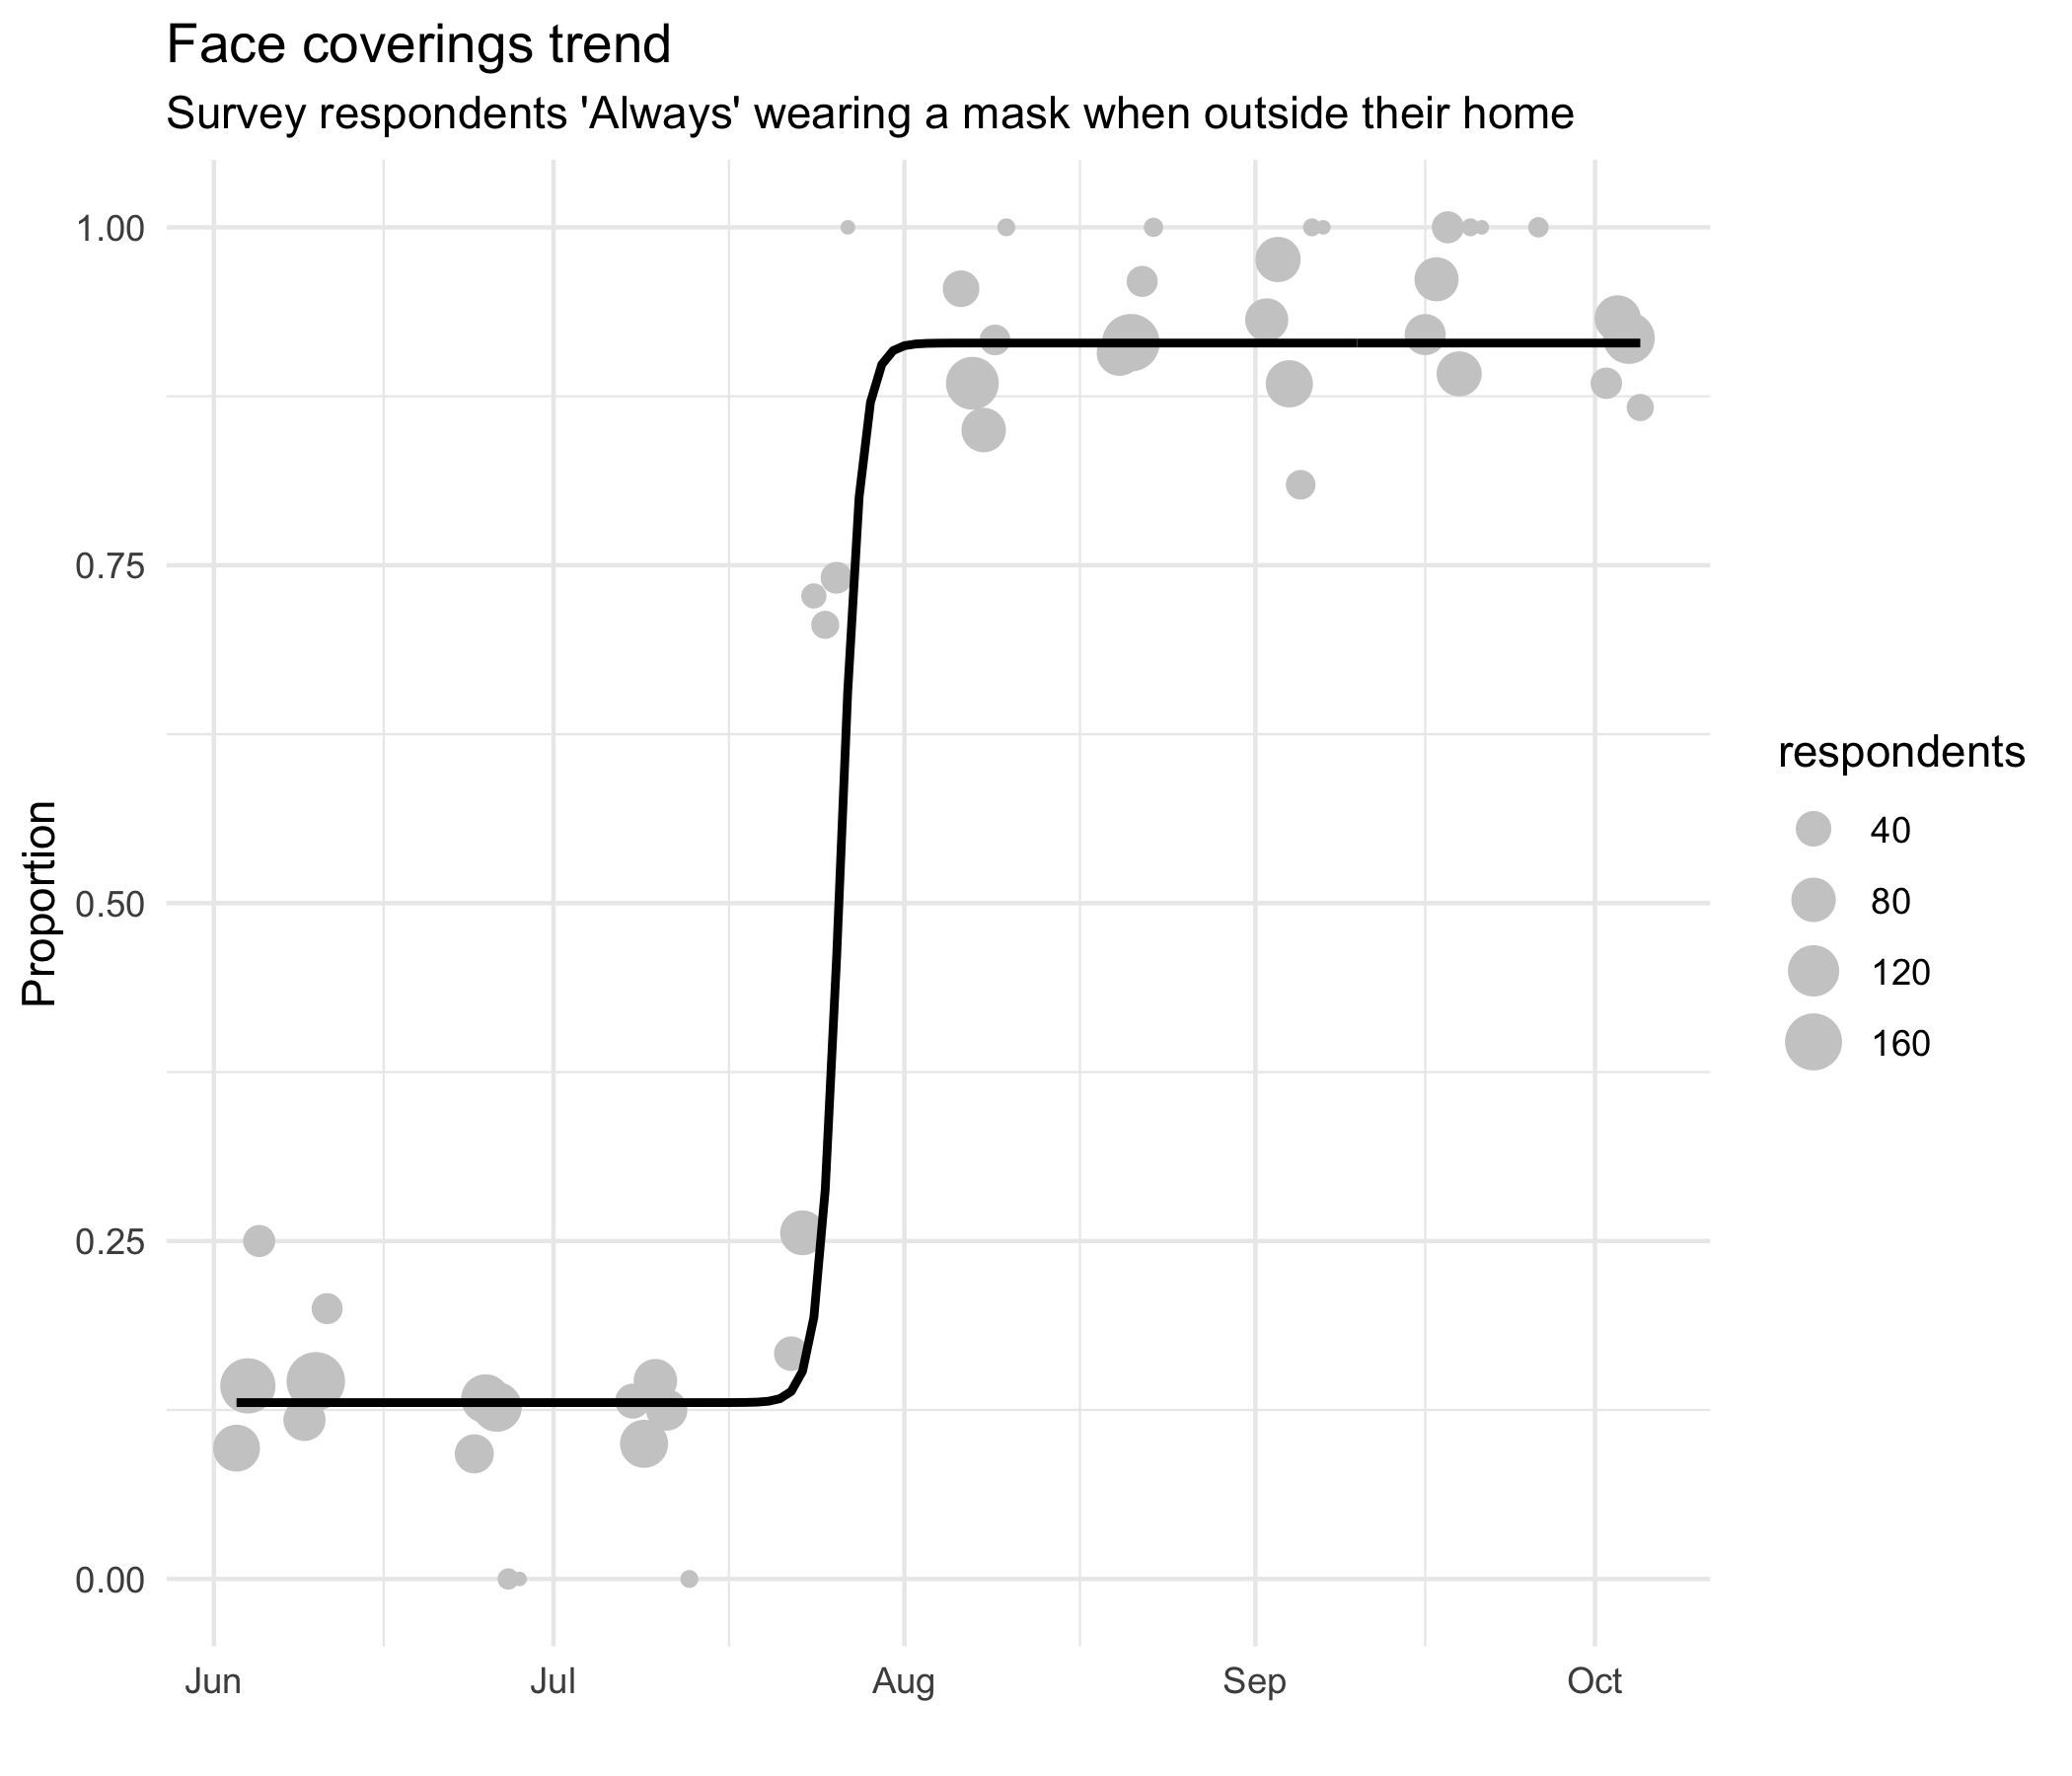
\includegraphics[scale=1]{../covid_19/projects/victoria/methods_figures/face_covering_fig.png}}
    \caption{Face coverings micro-distancing function for metropolitan Melbourne clusters with data used for fitting.}
	\label{fig:face}
\end{figure}

\section{Between cluster mixing}
The preceding section describes the creation of heterogeneous mixing matrices by age for each of the nine health service clusters individually. These mixing matrices are then combined to create a single time-varying heterogeneous mixing matrix by cluster and age resulting in a 144 by 144 (\(9\times16=144\)) square mixing matrix. The force of infection for an index cluster is calculated from the mixing matrices of the age-assortative matrix for each of the clusters modelled. For clusters other than the index cluster, the mixing matrices are multiplied by a parameter that represents the extent of inter-cluster mixing. This is then added to the mixing matrix for the index cluster multiplied by \(1-8\times intercluster\;mixing\) (because there are eight clusters other than the index cluster contributing to the mixing matrix) to create the final inter-cluster mixing matrix. The upper limit of prior of the \textit{intercluster mixing} parameter is set to be considerably less than one ninth, to ensure most of the force of infection is contributed from the index cluster (Table \ref{tab:calibration_params}).
